\chapter{Introduction to Sequences}

A sequence is a list of numbers in a particular order. \{1, 3, 5, 7, 
9\} is a sequence. So is \{$\frac{1}{2}$, $\frac{1}{4}$, $\frac{1}{8}$, 
$\cdots$\}. There are many types of sequences. We will present two of 
the most common types in this chapter: arithmetic and geometric 
sequences. 

Sequences are generally represented like this:
$$a_1, a_2, a_3, a_4,...,a_n,...$$

The first number, $a_1$, is called the \textit{first term}, $a_2$ is 
the \textit{second term}, and $a_n$ is the \textit{nth term}. A 
sequence can be finite or infinite. If the sequence is infinite, we 
represent that with ellipses ($\cdots$) at the end of the list, to 
indicate that there are more numbers. 

We can also write formulas to represent a sequence. Take the first 
example, the finite sequence \{1, 3, 5, 7, 9\}. Notice that each term 
is two more than the previous term. We can define the sequence 
\textit{recursively} by defining the $n^{th}$ term as a function of 
the $(n-1)^{th}$ term. In our example, we see that $a_n = a_{n-1}+2$ 
with $a_1 = 1$ for $1 \leq n \leq 5$. This is called a recursive 
formula, because you have to already know the $(n-1)^{th}$ term to 
find the $n^{th}$ term. 

Another way to write a formula for a sequence is to find a rule for 
the $n^{th}$ term. In our example sequence, the first term is 1 plus 
0 times 2, the second term is 1 plus 1 times 2, the third term is 1 
plus 2 times 2, and so one. Did you notice the pattern? The $n^{th}$ 
term is 1 plus (n-1) times 2. We can write this mathematically: $$a_n 
= 1 + 2(n-1)\text{ for } 1 \leq n \leq 5$$\\ 
This is called the \textit{explicit} formula because each term is 
explicitly defined. Notice that for the second way of writing a formula, 
we don't have to state what the first term is --- the formula tells us. 

\section{Arithemtic sequences}
Our first example sequence, \{1, 3, 5, 7, 9\} is a \textit{finite}, 
\textit{arithmetic} sequence. We know it is finite because there is a 
limited number of terms in the sequence (in this case, 5). How do we 
know it is arithmetic?

An arithmetic sequence is one where you add the same number every 
time to get the next term. Our example is an arithmetic sequence 
because you add 2 to get the next term every time. That number that 
you add is called the \textit{common difference}, so we can say the 
sequence \{1, 3, 5, 7, 9\} has a common difference of 2. The common 
difference can be positive (in the case of an increasing arithmetic 
sequence) or negative (in the case of a decreasing arithmetic 
sequence). Formally, we can find the common difference of an 
arithmetic sequence by subtracting the $(n-1)^{th}$ term from the 
$n^{th}$ term: 
$$d = a_n - a_{n-1}$$

\begin{Exercise}[label = seq1]
Which of the following are arithmetic sequences? For the arithmetic 
sequences, find the common difference.
\begin{enumerate}
\item \{$\frac{1}{2}$, $\frac{1}{4}$, $\frac{1}{6}$, $\frac{1}{8}$,...\}
\item \{5, 8, 11, 14, 17, ...\}
\item \{3, -1, -5, -9, ...\}
\item \{-1, 2, -3, 4, -5, 6, ...\}
\end{enumerate}
\end{Exercise}

\begin{Answer}[ref=seq1]
\begin{enumerate}
\item not arithmetic
\item arithmetic, common difference is 3
\item arithmetic, common difference is -4
\item not arithmetic
\end{enumerate}
\end{Answer}


\subsection{Formulas for arithmetic sequences}
If you are given an arithmetic sequence, you can write an explicit or 
recursive formula. You can think of the formula as a function where 
the domain (input) is restricted to integers greater than or equal to 
one. Let's write explicit and recursive formulas for the sequence 
\{3, -1, -5, -9, ...\}. 

For either type of formula, we need to identify the common difference. 
Since each term is 4 less than the previous term, the common 
difference is -4 (see figure \ref{fig:comdiff}). This means the 
$n^{th}$ term is the $(n-1)^{th}$ term minus 4. The general form of a 
recursive formula is $a_n = a_{n-1} + d$, where $d$ is the common 
difference. For our example, the common difference is -4, so we can 
write a recursive formula:
$$a_n = a_{n-1}-4$$

However, this formula doesn't tell us what $a_1$ is! For recursive 
formulas, you have to specify the first term in the sequence. So, the 
\textit{complete} recursive formula for the sequence is:
$$a_n = a_{n-1}-4$$
$$a_1 = 3$$

\begin{figure}[htbp]
\centering
    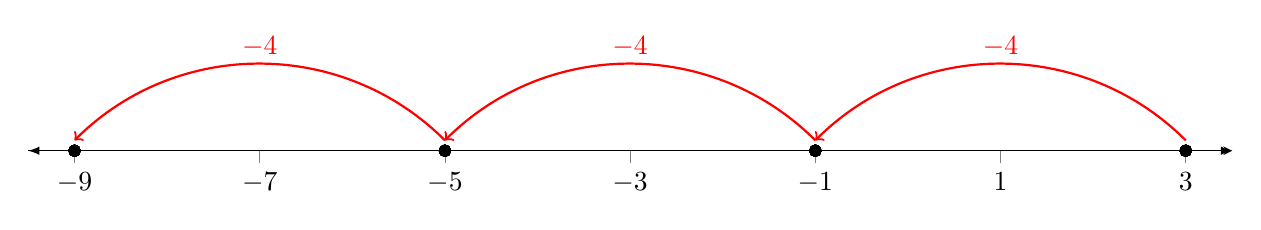
\begin{tikzpicture}
        \begin{axis}[axis y line = none, width = 2*\axisdefaultwidth, height = 0.25*\axisdefaultwidth, axis lines = center, xtick align = outside, xmin = -9.5, xmax = 3.5, xtick = {-9, -7, ...,3}, ymin = -0.5, ymax = 0.5, clip = false]
        \draw[latex-latex](-9.5,0) --(3.5, 0);
        \addplot[mark=*, black](-9, 0);
        \addplot[mark=*, black] (-5, 0);
        \addplot[mark=*, black] (-1, 0);
        \addplot[mark=*, black] (3, 0);
        \draw[->, red, thick](3, 0.25) to [bend right = 45] (-1, 0.25);
        \draw[->, red, thick](-1, 0.25) to [bend right = 45] (-5, 0.25);
        \draw[->, red, thick](-5, 0.25) to [bend right = 45] (-9, 0.25);
        \node[red] at (1, 2.5) {$-4$};
        \node[red] at (-3, 2.5) {$-4$};
        \node[red] at (-7, 2.5) {$-4$};
        \end{axis}
\end{tikzpicture}
    \caption{The common difference in the sequence \{3, -1, -5, -9,...\} is -4}
    \label{fig:comdiff}
\end{figure}

Recursive formulas make it easy to see how each term is related to 
the next term. However, it is difficult to use recursive formulas to 
find a specific term. Say we wanted to know the $7^{th}$ term in the 
sequence. Well, from the formula, we know that:
$$a_7 = a_6 - 4$$

What is $a_6$? Again, we see that
$$a_6 = a_5 - 4$$

Now we have to find $a_5$! If we keep going, we see that:
$$a_5 = a_4 - 4$$
$$a_4 = a_3 - 4$$
$$a_3 = a_2 - 4$$
$$a_2 = a_1 - 4$$

Since we were told $a_1$, we can find $a_2$ and propagate our terms 
back up the chain to find $a_7$:
$$a_2 = 3 - 4 = -1$$
$$a_3 = a_2 - 4 = -1 - 4 = -5$$
$$a_4 = a_3 - 4 = -5 - 4 = -9$$
$$a_5 = a_4 - 4 = -9 - 4 = -13$$
$$a_6 = a_5 - 4 = -13 - 4 = -17$$
$$a_7 = a_6 - 4 = -17 - 4 = -21$$

Ultimately, we see that $a_7 = -21$. That was a lot of work! You can 
imagine that for higher $n$ terms, such as the $100^{th}$ or 
$1000^{th}$ term, this method becomes cumbersome. This is where the 
explicit formula is more useful.

The general form of an explicit formula for an arithmetic sequence is 
$$a_n = a_1 + d \times (n-1)$$

where $d$ is the common difference. For our example sequence, \{3, -1, 
-5, -9, ...\}, the common difference is $-4$. So the explicit formula 
is
$$a_n = 3 + (-4)(n-1) = 3 - 4(n-1)$$

You may be tempted to distribute and simplify, which is fine and 
yields an equivalent formula:
$$a_n = 7-4n$$

Now, to find the $7^{th}$ term, all we have to do is substitute $n=7$:
$$a_7 = 3 - 4(7 - 1) = 3 - 4(6) = 3 - 24 = -21$$

We get the same answer with much less effort!

Another example of a recursive sequence is the Fibonacci sequence which we will cover in-depth later

\begin{Exercise}[label=seq2]
An arithmetic sequence is defined by the recursive formula $a_n = 
a_{n-1} + 5$ with $a_1 = -4$. Write the first 5 terms of the sequence 
and determine an explicit formula for the same sequence.
\end{Exercise}

\begin{Answer}[ref=seq2]
The first five terms are \{-4, 1, 6, 11, 16\} and an explicit formula 
is $a_n = -4 + 5(n-1)$. 
\end{Answer}

\begin{Exercise}[label=seq3]
The first four terms of an arithmetic sequence are \{$\pi$, 
$\frac{3\pi}{2}$, $2\pi$, $\frac{5\pi}{2}$\}. What is the common 
difference? Write explicit and recursive formulas for the infinite 
sequence.
\end{Exercise}

\begin{Answer}[ref=seq3]
The common difference is $\frac{3\pi}{2} - \pi = \frac{\pi}{2}$. The 
recursive formula is $a_n = a_{n-1} + \frac{\pi}{2}$ with $a_1 = \pi$. 
The explicit formula is $a_n = \pi + \frac{\pi}{2}(n-1)$. 
\end{Answer}

\section{Geometric sequences}
Let's look at the other sequence given as an example at the beginning 
of the chapter: \{$\frac{1}{2}$, $\frac{1}{4}$, $\frac{1}{8}$, 
$\cdots$\}. How is each term related to the previous term? Well, 
$\frac{1}{4}$ is half of $\frac{1}{2}$, and $\frac{1}{8}$ is half of 
$\frac{1}{4}$, so each term is the previous term multiplied by 
$\frac{1}{2}$. When each term in a sequence is a multiple of the 
previous term, this is a \textit{geometric} sequence. The number we 
multiply by each time (in our example, this is $\frac{1}{2}$), which is 
called the \textit{common ratio}. The common ratio can be positive 
or negative, but not zero. 

An easy way to determine the common ratio (r) is to divide the 
$n^{th}$ term by the $(n-1)^{th}$ term. In our example sequence, 
the first term is $\frac{1}{2}$ and the second is $\frac{1}{4}$. 
$$r = \frac{a_2}{a_1} = \frac{1/4}{1/2} = \frac{1}{2}$$

which returns the common ratio we already identified, $r= \frac{1}{2}$. 

If the common ratio is negative, then the sequence will "flip" back 
and forth from positive to negative. For example, suppose there is a 
geometric sequence such that $a_1 = 1$ and $r = -2$. Then the first 5 
terms are \{1, -2, 4, -8, 16\}. Whenever you see a sequence going 
back and forth from positive to negative, that means the common ratio 
is negative. 

For positive common ratios, if $r>1$, then the sequence is increasing. 
And if $r<1$, the sequence is decreasing. 

\subsection{Formulas for geometric sequences}
Like arithmetic sequences, we can write recursive and explicit 
formulas. For geometric sequences, the recursive formula has the 
general form: 
$$a_n = r(a_{n-1})$$

where r is the common ratio and $a_1$ is specified. For our example 
sequence, \{$\frac{1}{2}$, $\frac{1}{4}$, $\frac{1}{8}$, $\cdots$\}, 
the recursive formula is:
$$a_n = \frac{1}{2}a_{n-1}$$
$$a_1 = \frac{1}{2}$$

In a geometric sequence, each term is the first term, $a_1$, 
multiplied by the common ratio, r, $n-1$ times. Therefore, the 
general form of an explicit formula for a geometric function is:
$$a_n = (a_1)r^{n-1}$$

Again, for our example sequence, $a_1 = \frac{1}{2}$ and $r = 
\frac{1}{2}$, so the explicit formula is:
$$a_n = (\frac{1}{2})(\frac{1}{2})^{(n-1)}$$

\begin{Exercise}[label=seq4]
Which of the following are geometric sequences? For each geometric 
sequence, determine the common ratio.
\begin{enumerate}
\item \{2, -4, 6, -8,...\}
\item \{4, 2, 1, $\frac{1}{2}$, ...\}
\item \{-5, 25, -125, 525, ...\}
\item \{2, 0, -2, -4, ...\}
\end{enumerate}
\end{Exercise}

\begin{Answer}[ref=seq4]
\begin{enumerate}
\item not geometric
\item geometric sequence with common ratio $r = \frac{1}{2}$
\item geometric sequence with common ration $r = -5$
\item not geometric
\end{enumerate}
\end{Answer}

\begin{Exercise}[label=seq5]
A geometric sequence is defined by the recursive formula $a_n = a_{n-1} \times \frac{3}{2}$ with $a_1 = 1$. Write the first five terms of the sequence and determine an explicit formula for the same sequence. 
\end{Exercise}

\begin{Answer}[ref=seq5]
The first five terms are \{1, $\frac{3}{2}$, $\frac{9}{4}$, $\frac{27}{8}$, $\frac{81}{16}$\}. An explicit formula for this sequence is $a_n = 1(\frac{3}{2})^{(n-1)}$. 
\end{Answer}

\begin{Exercise}[label=seq6]
The first four terms of a geometric sequence are \{-4, 2, -1, $\frac{1}{2}$\}. What is the common ratio? Write recursive and explicit formulas for the infinite sequence. 
\end{Exercise}

\begin{Answer}[ref=seq6]
The common ratio is $\frac{a_{n}}{a_{n-1}} = \frac{2}{-4} = -\frac{1}{2}$. A recursive formula would be $a_n = a_{n-1} \times -\frac{1}{2}$ with $a_1 = -4$. An explicit formula would be $a_n = (-4)(-\frac{1}{2})^{(n-1)}$. 
\end{Answer}

















